\section{Additional results}
\label{app:tables}

\subsection{All methods on held-out Berka}
\begin{figure}[htbp]
\centering
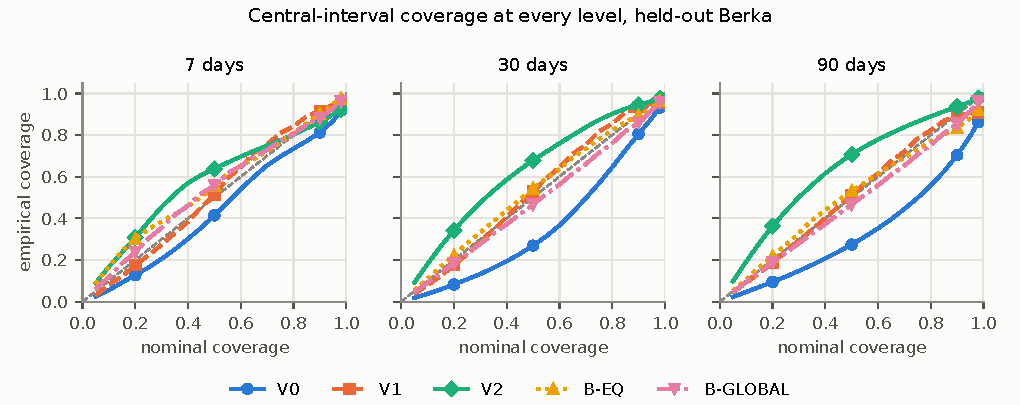
\includegraphics[width=\linewidth]{figures/coverage-heldout.pdf}
\caption{Empirical against nominal pooled coverage of central intervals at
every level of a fine grid, held-out Berka (\R{ho/var/V2/30/forecasts}
origins per horizon and method).}
\label{fig:coverage}
\end{figure}
\begin{table}[htbp]
\centering\footnotesize\setlength{\tabcolsep}{4pt}
\tab{heldout-main}
\caption{Held-out Berka, every method on the same
\R{ho/var/V2/30/forecasts} origins in \R{ho/var/V2/30/accounts} accounts
per horizon (days). Columns:
(1) pooled coverage of central intervals (\%);
(2) CRPS skill against B-SA+ as the mean of per-account ratios (positive:
lower CRPS than B-SA+);
(3) the share of PIT values in the outer two of ten bins (\%; a flat
histogram puts a fifth there).
B-SA is a point forecast, so its coverage is undefined (--). Pooled skills,
mean CRPS and intervals for V2's comparisons are in
Table~\ref{tab:pairwise}.}
\label{tab:heldout}
\end{table}
\begin{figure}[htbp]
\centering
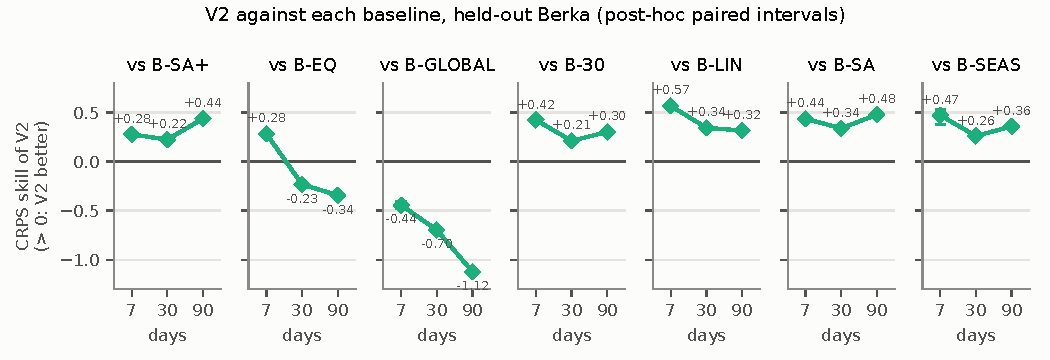
\includegraphics[width=\linewidth]{figures/skill-v2-heldout.pdf}
\caption{V2's account-mean CRPS skill against each baseline by horizon
(held-out, post hoc paired intervals).}
\label{fig:skill}
\end{figure}
\begin{table}[htbp]
\centering\scriptsize\setlength{\tabcolsep}{3.5pt}
\tab{heldout-strata}
\caption{Held-out strata: pooled \lC\% coverage (\%) and account-mean skill
against B-SA+ at \hB\ and \hC\ days. Origins and accounts are V2's in the
stratum. Strata are defined per origin, so an account can appear in more
than one stratum of a pair.}
\label{tab:strata}
\end{table}
\begin{table}[htbp]
\centering\footnotesize
\tab{devho-v2}
\caption{V2 on the development split (\R{dev/var/V2/30/forecasts} origins in
\R{dev/var/V2/30/accounts} accounts per horizon) and the held-out split
(\R{ho/var/V2/30/forecasts} in \R{ho/var/V2/30/accounts}). Coverage is
pooled; skill is the account mean.}
\label{tab:devho}
\end{table}
\begin{figure}[htbp]
\centering
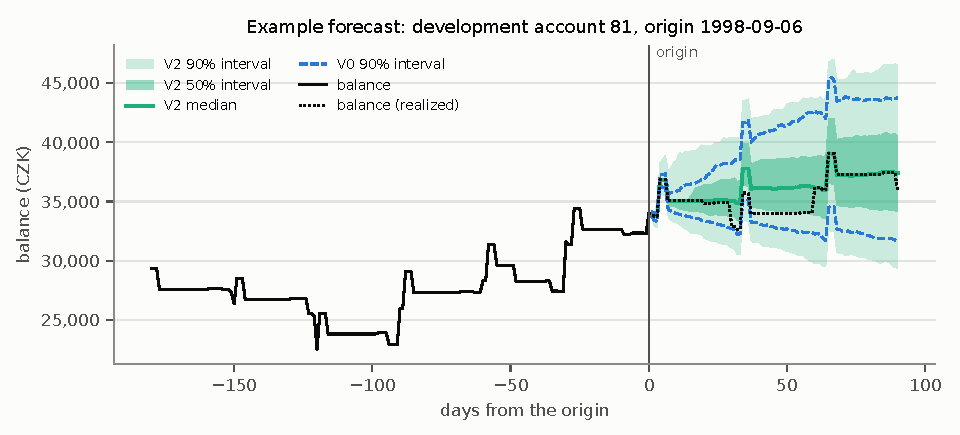
\includegraphics[width=0.85\linewidth]{figures/cone-example.pdf}
\caption{V2's and V0's \hC-day forecasts for development account
\R{fig/ex/account} at its last eligible origin (\R{fig/ex/origin}). The
account was chosen by a fixed rule (median record count among accounts with
detected income), not by look.}
\label{fig:cone}
\end{figure}

\subsection{Synthetic data: claims A1 and B2}
\paragraph{Claim A1 holds.} On model-matched data, with the protocol of the
engine's earlier calibration test, every central interval of V0 is within
the tolerance at every horizon (Appendix, Table~\ref{tab:a1}). With the
detector off, the \lC\% interval covers \R{syn/a1/no-detector/7/0.9/coverage},
\R{syn/a1/no-detector/30/0.9/coverage} and
\R{syn/a1/no-detector/90/0.9/coverage}\%. This is a correctness check: on
data drawn from its own model the filter is the right estimator, and
passing says little about usefulness.

\paragraph{The synthetic panel (claim B2).} Table~\ref{tab:synthetic}
gives \R{c/panel-seeds} seeds of \R{c/panel-days} days per generator,
\R{syn/data/realistic_origins} origins each.
\begin{itemize}
\item \textbf{V2 equals V0 here.} V2's sparse rule never fired on
  synthetic data (\R{d/syn-sparse} of \R{d/syn-origins} origins), because
  synthetic spending has many small transactions a day. Synthetic data
  therefore says nothing about V2's sparse model, which is exercised only
  on Berka. There the rule fired at every one of \R{ho/vdata/origins}
  held-out origins.
\item \textbf{The per-account baselines.} On the realistic generator, V0
  has lower CRPS than B-SA+ (account-mean skill \R{syn/re/V0/30/skill} and
  \R{syn/re/V0/90/skill} at \hB\ and \hC\ days) and than every
  per-account baseline.
\item \textbf{B-GLOBAL}, trained on \R{c/train-seeds} separate seeds of the
  same generator: the difference is not significant. The paired skill is
  \R{syn/rep/V0/B-GLOBAL/30/skill} [\R{syn/rep/V0/B-GLOBAL/30/skill_lo},
  \R{syn/rep/V0/B-GLOBAL/30/skill_hi}] at \hB\ days and
  \R{syn/rep/V0/B-GLOBAL/90/skill} [\R{syn/rep/V0/B-GLOBAL/90/skill_lo},
  \R{syn/rep/V0/B-GLOBAL/90/skill_hi}] at \hC\ days. B2 required an
  interval excluding zero, so it fails against B-GLOBAL. We set no
  equivalence margin, so this is not evidence that the two are
  equivalent.
\item \textbf{Model-matched data}: B-GLOBAL has lower CRPS at \hB\ days
  (\R{syn/mmp/V0/B-GLOBAL/30/skill}).
\end{itemize}

\begin{table}[t]
\centering\footnotesize
\tab{synthetic-main}
\caption{Synthetic panel: \R{c/panel-seeds} seeds per generator,
\R{syn/data/realistic_origins} origins per method and horizon. Pooled
coverage (\%) and account(seed)-mean skill against B-SA+. V2's sparse rule
never fired, so V2 equals V0. V3 was not run on synthetic data.}
\label{tab:synthetic}
\end{table}


\begin{table}[htbp]
\centering\footnotesize
\tab{synthetic-a1}
\caption{Claim A1: V0's pooled coverage (\%) on model-matched data with the
protocol of the engine's earlier calibration test (\R{c/a1-seeds} seeds,
three origins each). The numbers reproduce that test's output exactly.}
\label{tab:a1}
\end{table}

\subsection{Further exploratory checks (development only)}
\begin{itemize}
\item \textbf{A past-only drift rule.} An origin is kept only if its
  account's drift up to that origin stays within the threshold. This
  selects exactly the origins of the frozen full-history rule:
  \R{xd/s1/origins_p} against \R{xd/s1/origins_f}. Every drift-excluded
  account already drifts by at least \R{xd/s1/min_drift_at_a_grid_origin_of_an_excluded_account}
  crowns at its first possible origin.
\item \textbf{Who the minimum-history rules remove.} Origins failing the
  minimum-records rule have daily balance volatility of
  \R{xd/s1/groups/g3-failing-min-records-scale-defined/daily-sd-over-s/median}
  of a month's flow, against
  \R{xd/s1/groups/g3-eligible-origins/daily-sd-over-s/median} for eligible
  origins. They are few.
\item \textbf{The selection rule is robust.} Weighted by account instead of
  by origin, it still selects V2 (score \R{xd/s2/selection/V2/score_account_equal}
  against V1's \R{xd/s2/selection/V1/score_account_equal}).
\item \textbf{Origin phase.} On grids shifted by +10 and +20 days, every
  sign holds: V2 beats B-SA+, and B-EQ beats V2 at \hB\ and \hC\ days.
  B-EQ's pooled lead at \hB\ days shrinks, from
  \R{xd/s3/V2-vs-B-EQ/30/skill_pooled} on the frozen grid
  (\R{xd/s3/V2-vs-B-EQ/30/forecasts} origins) to
  \R{xd/s8-offset10/V2-vs-B-EQ/30/skill_pooled} and
  \R{xd/s8-offset20/V2-vs-B-EQ/30/skill_pooled}
  (\R{xd/s8-offset10/V2-vs-B-EQ/30/forecasts} and
  \R{xd/s8-offset20/V2-vs-B-EQ/30/forecasts}). The offset-0 rerun, on the
  first \R{xd/s8-offset0/V2-vs-B-EQ/30/accounts} development accounts only,
  was an identity check and is not a comparison.
\end{itemize}

\subsection{The detector ablation in V2 (exploratory, development)}
\label{app:detector}
Removing the detector costs V2 far more than V0 (\S\ref{sec:components}).
We checked for a bug before reading anything else (specification S9,
\texttt{paper/REVISION.md}). On all \R{xd/s9/V2-nodet-vs-V2/30/forecasts} development origins
(\R{xd/s9/V2-nodet-vs-V2/30/accounts} accounts):
\begin{itemize}
\item the four configurations (V0 and V2, each with and without the
  detector) reproduce the stored forecasts exactly;
\item the branch V2 uses (sparse spending) is the same with and without the
  detector at every origin;
\item V0 and V2 share the same filter state at every origin.
\end{itemize}
The effect is genuine. By stratum, pooled skill of the variant without the
detector against its full model, account mean in brackets (origins per
horizon in brackets after each stratum):

\begin{center}\scriptsize\setlength{\tabcolsep}{3pt}
\begin{tabular}{l ll ll}
\toprule
 & \multicolumn{2}{c}{V2 without detector} & \multicolumn{2}{c}{V0 without detector}\\
\cmidrule(lr){2-3}\cmidrule(lr){4-5}
Stratum & \hB\ d & \hC\ d & \hB\ d & \hC\ d\\
\midrule
income detected, income alarm (\R{xd/s9-inc-alarm/V2-nodet-vs-V2/30/forecasts}) & \pq{xd/s9-inc-alarm/V2-nodet-vs-V2}{30} & \pq{xd/s9-inc-alarm/V2-nodet-vs-V2}{90} & \pq{xd/s9-inc-alarm/V0-nodet-vs-V0}{30} & \pq{xd/s9-inc-alarm/V0-nodet-vs-V0}{90}\\
income detected, no income alarm (\R{xd/s9-inc-noalarm/V2-nodet-vs-V2/30/forecasts}) & \pq{xd/s9-inc-noalarm/V2-nodet-vs-V2}{30} & \pq{xd/s9-inc-noalarm/V2-nodet-vs-V2}{90} & \pq{xd/s9-inc-noalarm/V0-nodet-vs-V0}{30} & \pq{xd/s9-inc-noalarm/V0-nodet-vs-V0}{90}\\
no income detected (\R{xd/s9-noinc/V2-nodet-vs-V2/30/forecasts}) & \pq{xd/s9-noinc/V2-nodet-vs-V2}{30} & \pq{xd/s9-noinc/V2-nodet-vs-V2}{90} & \pq{xd/s9-noinc/V0-nodet-vs-V0}{30} & \pq{xd/s9-noinc/V0-nodet-vs-V0}{90}\\
\bottomrule
\end{tabular}
\end{center}

In the first stratum the forecast median at \hC\ days is biased by
\R{xd/s9/cb/inc-alarm/90/bias_V2-nodet} (normalized units) without the
detector, against \R{xd/s9/cb/inc-alarm/90/bias_V2} with it; V0's bias is
\R{xd/s9/cb/inc-alarm/90/bias_V0-nodet} and \R{xd/s9/cb/inc-alarm/90/bias_V0}.
The income alarms there fire early (median \R{xd/s9/mech/first-alarm-age/median}
days into the history; \R{xd/s9/mech/share-first-alarm-180/q25}\% of
origins have their first one within 180 days), because the first
income-tagged record is a median \R{xd/s9/mech/pay1-over-last/median}\% of
the later pay. With the detector, $\hat m$ is a median
\R{xd/s9/mech/m-det-over-last/median}\% of the last paycheck; without it,
\R{xd/s9/mech/m-nodet-over-last/median}\%. V0 is biased less; neither its
recorded lumps nor its spend-rate estimate accounts for the difference, so
the path by which V0 partly compensates is not identified.
